% chapter introduction 

\chapter{Introduction}
Grasping is one of the fundamental skills of human beings.  A three months old infant already possesses palmar grasp reflex. A baby closes his fingers when an object is placed in the palm. In the sixth month, the ability of active grasping is further developed. They can track an object with their eyes and grasp them actively. Gradually, they gain how to hand over an object between the left and the right hand. From eighth to ninth month, they can already perform precision grasping by only two fingers.  A ten months old infant already has some ability to perform task oriented grasping. They know how to grasp a nipple or a nursing bottle correctly so that they can suck them after grasping. As we can see, a human develops its grasping ability in the very early age, from the passive grasping reflex to the active grasping skill with task intention and accuracy. 

By contrast, the most advanced robots  can not reach the dexterity of grasping comparing to a human. In the factory, robots are designed to work in a structured environment. They have perfect knowledge of what type of objects they are working with, how the objects should look like,  when and where they should appear. Therefore, they can perform a range of manipulation tasks with high speed. These include material handling, manufacture ,etc.  Without these prior knowledge while operating robots in unstructured environment, grasping is a very challenging task for robots. People may ask why grasping is fairly a simple task even for little children but difficult to robots. In unstructured environment with little prior knowledge, robotic grasping is an interdisciplinary problem, which requires mastering of several tasks. These include object perception, reasoning about grasp configuration and robust control of grasp execution. 

\section{A brief history of research on robotic grasping}
The research on robotic grasping has a long history. Most researchers in the earliest time address the problem through analytic approaches. Previous work regarding contact models (\cite{Salisbury1983},\cite{Sinha1992}),  form/force closure (\cite{Dizioglu1984},\cite{Nguyen1988}), force optimizations(\cite{Buss1996},\cite{Liu2004})etc. lay the theoretical framework of determining a firm grasp. The stability of a grasp is usually quantified by a  quality metric (\cite{roa2015grasp},\cite{Borst2004}). The quality metric describes how much external wrench a grasp can resist. Bicchi and Kumar~\cite{Bicchi2000} provides a comprehensive survey of these methods. 

Using a simulator can, in general, accelerate algorithms designed to work on real robots. In the grasping community, there was no simulator until the emergence of `\textit{GraspIt}'~\cite{Miller2004}.  The `\textit{GraspIt}' simulator provides a fast collision detection and contact determination interface. It is designed for grasp planning with arbitrary objects and gripper types. Since then, a lot of grasp synthesis approaches (\cite{Miller1999},\cite{Kragic2001},\cite{Miller2003}) have been developed based on this tool. However, it remains a challenge to apply these approaches for grasping real objects, because most of them rely on prior knowledge of a given object model. Obviously, it is not feasible to create models  for every particular item in the world. In addition, due to the imperfection of real sensors, the perception of a robot usually contains estimation error, which further influence the grasping success. These approaches can not handle the problem of this kind.

Recently, with the development of sensing technologies, low-cost sensors for acquiring rich 3D information of environment is available. Data-driven methods become familiar and put more emphasis on perception for grasping. Different from analytic approaches, they focus on extracting information from the sensor input, which is relevant for the synthesis of a grasp. These include object representations, extraction of grasp relevant features and reactive grasp executions. These methods can better handle the perception uncertainty which is essential for the real grasping problem. A comprehensive review of data-driven methods is given by Bohg et al.~\cite{Bohg2014}.

 
\section{Challenges}
Although robotic grasping has been studied intensively in the past, it remains a gap between the theoretical findings and technical realization in a real environment. Various models and methods have been proposed to  find feasible grasp configurations. However, there are only a few methods which both consider how to generate task orientated grasp configuration and exploit the robot kinematics simultaneously. In addition, most object representations designed for grasp synthesis simply use a mesh model for grasp synthesis, which is not able to integrate perceptual uncertainty. Methods that able to handle the perceptual uncertainty probabilistically and model the object efficiently is missing. Furthermore, an integrated system solution for taking advantage of a robot's structure while considers the perceptual uncertainty, and allows a robust adaptive grasp execution is not available. The various aspects of challenges for robotic grasping are summarized in this section. 

\subsubsection{How to design a task-oriented grasping skill which is reusable for mobile manipulation tasks?}

In a mobile manipulation scenario such as assembly work, a robot is required to assemble several objects together. The robot usually has to perform a sequence of manipulation actions, which include grasping, placing, insertion and so on. According to a given assembly plan, one object may be picked and placed multiple times, so that the orientation of the object meets the condition of other manipulation steps. Therefore, grasping serves as one of the core skills for the task. It is preferred to have a reusable grasping skill which can be easily used throughout the entire manipulation steps. In addition, grasping has also to be task-oriented. For an object and a given gripper, it may exist thousands of grasp configurations which are feasible, but only a sub-set of these configurations meet both  task constraint and workspace constraint. How to calculate a `good' robot configuration for grasping is an issue.  Another problem regarding this scenario is the objects to be assembled may locate freely at a wide range of area. The robot must use its mobility to move to positions so that the objects are reachable. Determining these intermediate base positions which minimize the movement of the robot while combining the base motion and manipulator motion can increase the overall task performance. It remains a big challenge how to address the above-mentioned issues in an integrated framework. 

\subsubsection{How to model a grasping favorable object representation and use it for precision grasp synthesis?}

A large portion of objects daily life have irregular shapes. To handle the variety of object's form is a challenge. One na\"ive approach for representing such objects is by approximating the geometry by  shape primitives. This representation may feasible for power grasping such as caging, but is not suitable for precision grasping with fingertips. For tasks which require precision, choose of an appropriate representation for grasp synthesis is an issue because the accuracy of where to establish contact is crucial to grasp success. A good representation should be able to model the surface as accurate as possible. If the object model is not known in prior, the representation should allow fast reconstruction online. In addition, as the object model can never be perfect, the representation should model the uncertainty of the surface, so that the robot is able to estimate the probability of success. Furthermore, for grasp synthesis, it is often required to evaluate a large number of grasp hypothesis, fast access of surface element for computing the contact normals can accelerate the speed of finding a feasible grasp configuration. It is a big challenge to design such a representation which can include all the mentioned features and a grasp synthesis method that is tailored for the representation. 

\subsubsection{How to increase the robustness of grasp execution in spite of perceptual uncertainty?}
Grasp execution refers to the actual motion of performing a grasp. Traditional approaches usually execute pre-computed grasp movements in open loop. However, due to perceptual uncertainty, the planned grasping points may different from actual contact points, performing of the scheduled grasp trajectory may result in failure. As perceptual uncertainty always exists, the challenge remains how to reduce the uncertainty even an initial grasp hypothesis is given. One approach to increasing the robustness of grasping is by closing the perception-action loop during the grasp execution. The robot is required to adapt its grasp motion to the perceptual result. For a mobile manipulator, how to coordinate and control the required component to achieve such adaptive grasp behavior is a big challenge.   


\section{Main contributions and outline of this thesis}
In this dissertation, a general and integrated system is developed to tackle the challenges as mentioned above for robotic grasping. Three grasping scenarios which represent different aspects of grasping are explored. Fig.~\ref{fig:outline} illustrates the outline of this thesis. In chapter~\ref{chapter2}, we propose to unify various aspects of challenges using a Bayesian network. The variables defined in the model represent factors which are relevant to the overall grasping success. The difference between the scenarios only exist in which variables are observable. In chapter~\ref{chapter4}, we focus on how to generate reusable task-oriented grasping skills for assembly task. For this purpose, a skill-based framework is proposed so that a mobile manipulator can perform the assembly task very efficient and flexible. Different from the objects that are known in prior in an assembly tasks, we address the problem of unknown object grasping in chapter~\ref{chapter:gs}. A grasp synthesis method based on a novel probabilistic object representation is proposed in this chapter. The method improves the accuracy of grasping significantly. In chapter~\ref{chapter_control}, we tackle another grasping scenario that the accuracy of sensor used for grasping is not high. To face the challenge, an adaptive grasping control architecture is proposed so that the robot is able to adapt its grasping motion online during execution. In this way, robust grasp execution is achieved despite sensing uncertainty. 
\begin{figure}[!htbp]
\centering

\includegraphics[width=0.7\linewidth]{outline.pdf}
\captionsetup{justification=raggedright}
\caption{Thesis outline}
\label{fig:outline}
\end{figure} 
\subsubsection{A skill framework for assembly problem exploiting arm-base coordination}
Mobile manipulators are the robots which equipped with a mobile base platform 
for navigation and arm(s) for manipulation. For reach-and-grasp tasks, state-of-the-art 
approaches consider it as two isolated problems: a navigation problem followed by a motion 
planning problem. Using these approaches a robot should first move its mobile platform 
to a location that the object is reachable, then use its manipulator to accomplish the object grasping task. Although it is a feasible solution, the time used to perform this task is not efficient. In contrast, a human performs the same task with all his actuation capability (arm, hand, body, locomotion) in a coordinated manner. In chapter~\ref{chapter4}, inspired by the human, we propose to bridge the gap between human reach-and-grasping and robotic reach- 
and-grasping by arm-platform coordination. An analysis of the reachability 
of a mobile manipulator is first conducted. The result revealed that the overlap between 
the workspace of a manipulator with the observation space of a fixed mounted camera is 
very limited. As a result, a mobile manipulator has to  face the following dilemma usually, 
the target object is located in the field of view of the robot, but it is not reachable from 
the robot manipulator, or the object is reachable from the manipulator but lies out of 
the field of view of the robot. This situation implies that arm-platform coordination is the only 
promising approach to solve the reach-and-grasping problem efficiently. To enable a mobile 
manipulator to move with its full degree of freedom (DOF), we propose a concept of 
virtual joints as well as a virtual kinematic chain. The virtual kinematic chain is composed of both the 
manipulators' joints and virtual joints. In this way, the planning of the arm- 
platform coordinated motion can be seamlessly integrated into an existing motion planning 
framework. We demonstrate the benefits of this concept in an assembly problem and propose a skill-based framework to solve the problem in a generalizable fashion. In this framework, reusable high-level skills can be parametrized to perform pick, place and insert operations. The high-level skills can reason about where to grasp the object so that the constraints for place and insert operation are satisfied. Fig.~\ref{fig:skill_over_view} illustrates the input and output of the system.
\begin{figure}[!htbp]
\centering
\includegraphics[width=0.8\linewidth]{skills_overview.pdf}
\captionsetup{justification=raggedright}
\caption{(a) A high-level assembly sequence provided to the system. P.R: The skill for picking and placing an object in another orientation. P.I: The skill for picking an object and inserting in another one. (b) A mobile manipulation robot performs the assembly task autonomously.}
\label{fig:skill_over_view}
\end{figure} 
\subsubsection{A probabilistic approach to the grasp synthesis for unknown objects }
The uncertainty of the real world, dynamics of objects and error in a perceptional 
system makes a robot difficult to guarantee that a grasp action will always lead to a 
success. To manage the complexity and uncertainty in the real world, modeling the success probability of a grasping action is a promising method to handle these problems. In chapter~\ref{chapter:gs}, the success probability is calculated based on a model of conditional grasping success and a model of object posterior. This method reduces the complexity of directly modeling the grasp success probability. It splits a complex model into two independent models which are not correlated with each other. The conditional grasping success model describes the probability of success by taken an action, under the condition that the object state is given. It is modelled using four criteria, which maps the principle of underlying grasp physics, actuation error and representation uncertainty to the model. Object posterior models the object state distribution after a series of observations are obtained. Depending on the choice of the representation, for some real world objects whose shape can be approximated by a group of shape primitives, the dimension of the object state space is small. The object posterior of these objects can be computed by e.g. Bayes filtering. For most real world objects, the dimension of state space is large because of their individual courses of the surface. We propose a new surface representation and a fusion method to compute the object posterior. The underlying structure of the surface representation is a variance augmented signed distance function. This representation allows temporal and spatial fusion by multiple depth cameras with individual noise characteristics. The result of the sensor fusion is a uncertainty-aware surface distribution which approximates the object posterior. After modeling the grasp success probability, the aim is to search for a grasp action that maximizes the success probability. For this purpose, we propose a simulated annealing method to find a feasible grasp. This approach seamlessly connects grasp perception and grasp control in a systematic way, while serves as a foundation for grasping unknown objects. The computational time of our method performs 30 times faster than a state-of-the-art method which uses a similar representation. Experimental results verify a significant grasping accuracy improvement in the scenario of grasping real world unknown objects by using the proposed method. Fig.~\ref{fig:synthesis_overview} elaborates some detail of proposed  method. 
\begin{figure}[!htbp]
\centering
\includegraphics[width=0.8\linewidth]{synthesis_overview.pdf}
\captionsetup{justification=raggedright}
\caption{(a) The object is presented to the robot for the first time. (b) The robot reconstructs the object surface by fusing sensor measurement from two depth cameras. (c) An uncertainty-aware object model is constructed and a feasible grasp is found for grasping the object. (d) Successful execution of the grasp on a real robot.}
\label{fig:synthesis_overview}
\end{figure} 
\subsubsection{An adaptive control architecture for closed-loop grasp execution}
Chapter~\ref{chapter_control} addresses the control aspect of the grasping process. In general, individual actuators of a mobile manipulator are usually controlled by their independent interface. However, arm-platform coordination requires control commands to be sent to each actuator simultaneously. To control the individual actuators in synchrony, we propose a system control architecture, which enables a plug-in mechanism to combine arbitrary independent actuators into a standard control loop in a flexible manner. This allows a mobile manipulator to easily switch and combine the actuators according to the requirements of a grasping phase. For example, a mobile manipulator can use arm-platform coordination in the pre-grasp phase for moving to a reachable position and for interacting with an object. Motions executed by the arm alone can be employed in the grasp-motion phase for approaching a grasp configuration. Arm-gripper coordination can be utilized in the force-closure phase for  stabilizing the object within the gripper. In most previous approaches, motions of the grasping are usually planned beforehand. Thus, the adaptation of the grasp motion to the change of the object state is not possible. We propose to solve this problem by an online trajectory generation algorithm and feed the state of the object back to the trajectory generator. In this way, a large control loop is closed by the system. Using the proposed method, a mobile manipulator is not only able to reason about the grasp configuration but also recognize the change of the environment and adapt to the change. As a result, the robustness of the grasping accuracy is significantly improved. In Fig.~\ref{fig:control_overview}, the robot uses the proposed method to grasp light objects. 
\begin{figure}[!htbp]
\centering
\includegraphics[width=0.6\linewidth]{control_overview.pdf}
\captionsetup{justification=raggedright}
\caption{(a) The robot is about to grasp light objects. The radius and position of the objects are estimated online during the reach-to-grasp phase. (b) The robot successfully pick up the object despite of large sensing uncertainty.}
\label{fig:control_overview}
\end{figure} 

%\subsubsection{Probabilistic modeling and Maximization of Grasping Success}
%Uncertainty of the real world, unknown dynamics of objects and error in a perceptional system makes a robot difficult to guarantee that a grasp action will  always lead to a success. To manage the complexity and uncertainty in the real world, modeling the success probability of a grasping action is a promising method to handle these problems. In Chapter 3 we describe a probabilistic approach to model the grasping process. The success probability is calculated based on a model of conditional grasping success and a model of object posterior. This method reduces the complexity of directly modeling the grasp success probability. It splits a complex modeling problem into two independent models which are not correlated with each other. The conditional grasp success model describes the probability of success by taken an grasp action, under the condition that the object state is given. It is modelled using four criteria, which maps the principle of underlying grasp physics, actuation uncertainty, representation uncertainty and a task  affordance to the model. Object posterior models the object state distribution after a series of observations are conducted. Depending on the choice of the representation, for some real world objects whose shape can be approximated by a group of shape primitives, the dimension of the object state space is small. The object posterior of these objects can be computed by e.g. Bayes filtering. For most real  world objects, the dimension of state space is large because of their individual courses of the surface, we propose a new surface representation and fusion method to compute the posterior. The underlying structure of the surface representation is a variance augmented signed distance function. This representation allows temporal and spacial fusion by multiple depth cameras with  individual noise characteristics. The result of the sensor fusion is a uncertainty-aware surface distribution which approximate the object posterior. After modeling the grasp success probability, the aim  is to search for a grasp action that maximizes the success probability. For this purpose, we propose a Monte Carlo based method to find an optimal grasp trajectory. This method seamlessly connects grasp perception and grasp control in a systematic way, while serves as a foundation for grasping unknown objects. The computational time of our method performs 30 times faster than the state-of-the-art. Experimental results verifies a significant grasping accuracy improvement in the scenario of  grasping real world unknown objects by using the proposed method. 
%
%
%\subsubsection{Arm-platform Coordination Enables Realizing Grasping Strategy and Efficient Mobile Manipulation}
%Mobile manipulators are the robots which typically equipped with a mobile base platform for navigation and arm(s) for manipulation. For reach-and-grasp tasks, state-of-the-art approaches consider it as two isolated problems: a navigation problem followed by a motion planning problem. Using these approaches a robot should first move with mobile platform to a location that the object is reachable, then use its manipulator to accomplish the object grasping task. Although it is a feasible solution, the time used to perform this task is not efficient. In contrast, a human performs the same task with all his actuation capability (arm, hand, body, locomotion) in a coordinated manner. In chapter 4, inspired by the human, we propose to bridge the gap between human reach-and-grasping and robotic reach-and-grasping by arm-platform coordination. In this chapter, an analysis of the reachability of a mobile manipulator is first conducted. The result revealed that the overlap between the workspace of a manipulator with the observation space of a fixed mounted camera is very limited. As a result, a mobile manipulator has to usually face the following dilemma, the target object is located in the field of view of the robot, but it is not reachable from the robot manipulator, or the object is reachable from the manipulator but lies out of the field of view of the robot. This implies that arm-platform coordination is the only promising approach to  efficiently solve the reach-and-grasping problem. To enable a mobile manipulator to move with its whole degree of freedom (DOF), we propose a concept of virtual joints, and add another kinematic structure by composing the virtual joints and the manipulators' joints into a common kinematic chain. In this way, the planning of the arm-platform coordinated motion can be seamless integrated into an existing motion planning framework. We demonstrate the benefits of this concept in two problems: grasp strategy planning and assembly task planning. In grasp strategy planning, we propose to design several strategies for the grasping process. Some are indented for reducing perceptual uncertainty, others are better for increasing grasp efficiency. A strategy selection algorithm based on Markov Decision Process is proposed to handle which strategy should be selected. In assembly task planning, two high-level assembly skills are designed to encapsulate low-level perception and motion planning tasks. A base-position planning algorithm based on iterative inverse kinematic is proposed to compute the optimal base placement to solve the aforementioned dilemma. The concept of arm-platform coordination allows a complex grasp strategy being executable in the strategy planning problem while improves the task efficiency for complex assembly problems.   
%
%
%\subsubsection{Boosting Grasping Robustness and Flexibility by an Adaptive Control Architecture}
%After the concept of arm-platform coordination is introduced in chapter 4. Chapter 5 addresses the control aspect of the grasping process. In general, individual actuators of a mobile manipulator are usually controlled by their independent interface. However, arm-platform coordination requires control commands to be sent to each actuator simultaneously. To control the individual actuators in synchrony, we propose a system control architecture, which enables a plug-in mechanism to combine arbitrary independent actuators into a common control loop in a flexible manner. This allows a mobile manipulator to easily switch and combine the actuators according to the requirements of a grasping phase. For example, a mobile manipulator can use arm-platform coordination in the pre-grasp phase for moving to a reachable position and for interacting with an object. Motions executed by arm alone can be used in the grasp-motion phase for approaching a grasp configuration. Arm-gripper coordination can be exploited in the force-closure phase for stabilizing the object within the gripper. 
%
%In the most state-of-the-art grasping approaches, motions of the grasping are usually pre-planned. Thus, adaptation of the grasp motion to the change of the object state is not possible. We propose to solve this problem by an online trajectory generation algorithm and feed the state of the object back to the trajectory generator. In this way, a large control loop is closed for the system. Using the proposed method, a mobile manipulator is not only able to reason about the grasp configuration  but also recognize the change of the environment and adapt to the change. As a result, the robustness of the grasping accuracy is significant improved. 

 

